% +++
% sequence = ["latex", "bibtex", "latex", "latex"]
% [programs.latex]
% 	command = "lualatex"
% 	opts = ["-synctex=1", "-file-line-error", "-interaction=nonstopmode"]
% 	args = ["%S"]
% [programs.bibtex]
% 	command = "upbibtex"
% 	target = "../ref.bib"
% 	args = ["%B"]
% +++

\documentclass[./main]{subfiles}
\graphicspath{{\subfix{./figures/section5/}}}
\setcounter{section}{4}

\usepackage{multicol}

\begin{document}

\newcommand{\sumSquare}[2]{%
  \directlua{
    function sum_square(x,y)
      if x > y then
        x, y = y, x
      end
      local s = 0
      for i = x, y do
        s = s + i^2
      end
      tex.sprint(math.floor(s))
    end
  }
  \directlua{ sum_square(#1,#2) }%
}



\begin{luacode*}
  function my_displace(str_before, str_after, sentence)
    local sentence_after = ""
    local l = #str_before - 1
    local i = 0
    while true do
      if string.sub(sentence, i, i+l) == str_before then
        sentence_after = sentence_after .. str_after
        i = i + l
      else
        sentence_after = sentence_after .. string.sub(sentence, i, i)
      end
      -- tex.sprint(i..",")
      i = i + 1
      if i > #sentence then
        break
      end
    end
    tex.sprint(sentence_after)
  end
\end{luacode*}
\newcommand{\displace}[3]{
  \directlua{ my_displace("#1","#2","#3") }%
}





\section{ちょっとしたTips}
\addtocontents{lof}{\protect\addvspace{1em}}
\noindent
ここまでで,基本的な\TeX の実行について幾分イメージがつきやすくなったと思う.
これより先は「へえ、そうだったのか」と個人的に思ったような\TeX 周りの何事かを完全に備忘録として記していく.

\subsection{\LuaLaTeX でなんとやら}
\subsubsection{フォント}
\noindent
本資料でもフォントの調整は行っている.
このように途中で変えるのもお手の物である.
\begin{table}[htbp]
  \caption{Fonts used in this document.}
  \label{tbl:fonts}
  \centering\begin{tabular}{rl}\bhline{1pt}
    Usage & Font Name \\\hline
    English main & TeX Gyre Termes\\
    Japanese main & Hiragino Mincho ProN\\
    English sans serif  & Verdana\\
    Japanese sans serif & Hiragino Kaku Gothic Pro\\
    Typewriter & New Computer Modern Mono10\\
    Footer & 3270 Narrow\\
    English in \verb|section| and \verb|subsection| & American Typewriter \\\bhline{1pt}
  \end{tabular}
\end{table}

\subsubsection{Luaコード}
\noindent
\LuaLaTeX の大きな特徴の一つはもちろん``Lua''である.
Luaは,高速な動作と高い移植性,組み込みの容易さが特徴であるスクリプト言語である\supercite{Lua_Wikipedia,Lua_intro}.
派生のLuaJITは動的型付けのスクリプト言語で最速言語である(らしい).

そんな高速なLuaを\TeX にからめて使っていく\supercite{Luaコツ,プログラミングwtTeX,pattern_syn_lua,Lua_challenge}.
もちろんプログラム言語なので普通に計算を行うことができて,わざわざ別のなにかを立ち上げることなく,計算して結果を出すことができる.例えば
\begin{center}
  \vspace{-7pt}
  \verb|$\sqrt{2}=$ \directlua{tex.sprint(math.sqrt(2))}|\\
  \vspace{-7pt}
\end{center}
などと書けば
\begin{center}
  \vspace{-7pt}
  $\sqrt{2}=$ \directlua{tex.sprint(math.sqrt(2))}\\
  \vspace{-7pt}
\end{center}
と表示される.

他にも引数を持つ自作関数を\verb|\newcommand|でつくると,本文中で\verb|\sumSquare{}{}|と書く度に,引数の小さい方から大きい方までの整数二条和を計算させられる.
\begin{figure}[h]
\centering
\begin{minipage}{0.35\linewidth}
  \begin{lstlisting}[emph={\\sumSquare,sumSquareFunc}]
\newcommand{\sumSquare}[2]{%
  \directlua{
    function sumSquareFunc(x,y)
      if x > y then
        x, y = y, x
      end
      local s = 0
      for i = x, y do
        s = s + i^2
      end
      tex.sprint(math.floor(s))
    end
  }%
  \directlua{ sumSquareFunc(#1,#2) }%
}
\end{lstlisting}
\end{minipage}
\begin{minipage}{0.45\linewidth}
  \centering\begin{tabular}{ll}
    \verb|\sumSquare{1}{10}| & \hspace{-2ex}$=\sumSquare{1}{10}$\\
    \verb|\sumSquare{-2}{1}| & \hspace{-2ex}$=\sumSquare{-2}{1}$\\
    \verb|\sumSquare{50}{-50}| & \hspace{-2ex}$=\sumSquare{50}{-50}$\\
  \end{tabular}
\end{minipage}
\end{figure}

もちろん文字列も扱える.
もし間違えて猫を犬にしてしまったときは,以下の自作関数\verb|\displace|を用いて,\verb|\displace{dog}{cat}{dog cat dog cat}|と書けば,``dog cat dog cat''を``\displace{dog}{cat}{dog cat dog cat}''と猫だらけにできる.
\begin{figure}[htbp]
\centering
\begin{minipage}{0.65\linewidth}
  \centering
  \vspace{-3pt}
  \begin{lstlisting}[emph={\\displace,myDisplace}]
\begin{luacode*}
  function myDisplace(str_before, str_after, sentence)
    local sentence_after = ""
    local l = #str_before - 1
    local i = 0
    while true do
      if string.sub(sentence, i, i+l) == str_before then
        sentence_after = sentence_after .. str_after
        i = i + l
      else
        sentence_after = sentence_after .. string.sub(sentence,i,i)
      end
      i = i + 1
      if i > #sentence then break end
    end
    tex.sprint(sentence_after)
  end
\end{luacode*}
\newcommand{\displace}[3]{ \directlua{myDisplace("#1","#2","#3")} }
\end{lstlisting}
\end{minipage}
\end{figure}


\clearpage
\LuaLaTeX はLuaを\LaTeX と絡めて使えるため,文書の様式・組版を変えることもできる.

\begin{figure}[htbp]
\begin{minipage}{0.6\linewidth}
\begin{lstlisting}[emph={vibrateLine}]
\documentclass[twocolumn]{article}
\usepackage{lipsum}
\usepackage{luacode}
\setlength{\columnsep}{1cm}
\pagestyle{empty}

\begin{luacode*}
vibrateLine = function (head, group, size)
  i = 1.5
  for list in node.traverse(head) do
    i = i + 0.13
    if list.id == node.id("hlist")
    then
      list.shift = list.shift - (1200000 * (math.sin (i)))
    end
  end
  return head
end
\end{luacode*}

\directlua{%
  luatexbase.add_to_callback('vpack_filter',vibrateLine,"strict")%
}

\begin{document}
  \lipsum[1-10]
\end{document}
\end{lstlisting}
\end{minipage}
\hfill
\begin{minipage}{0.35\linewidth}
  \centering
  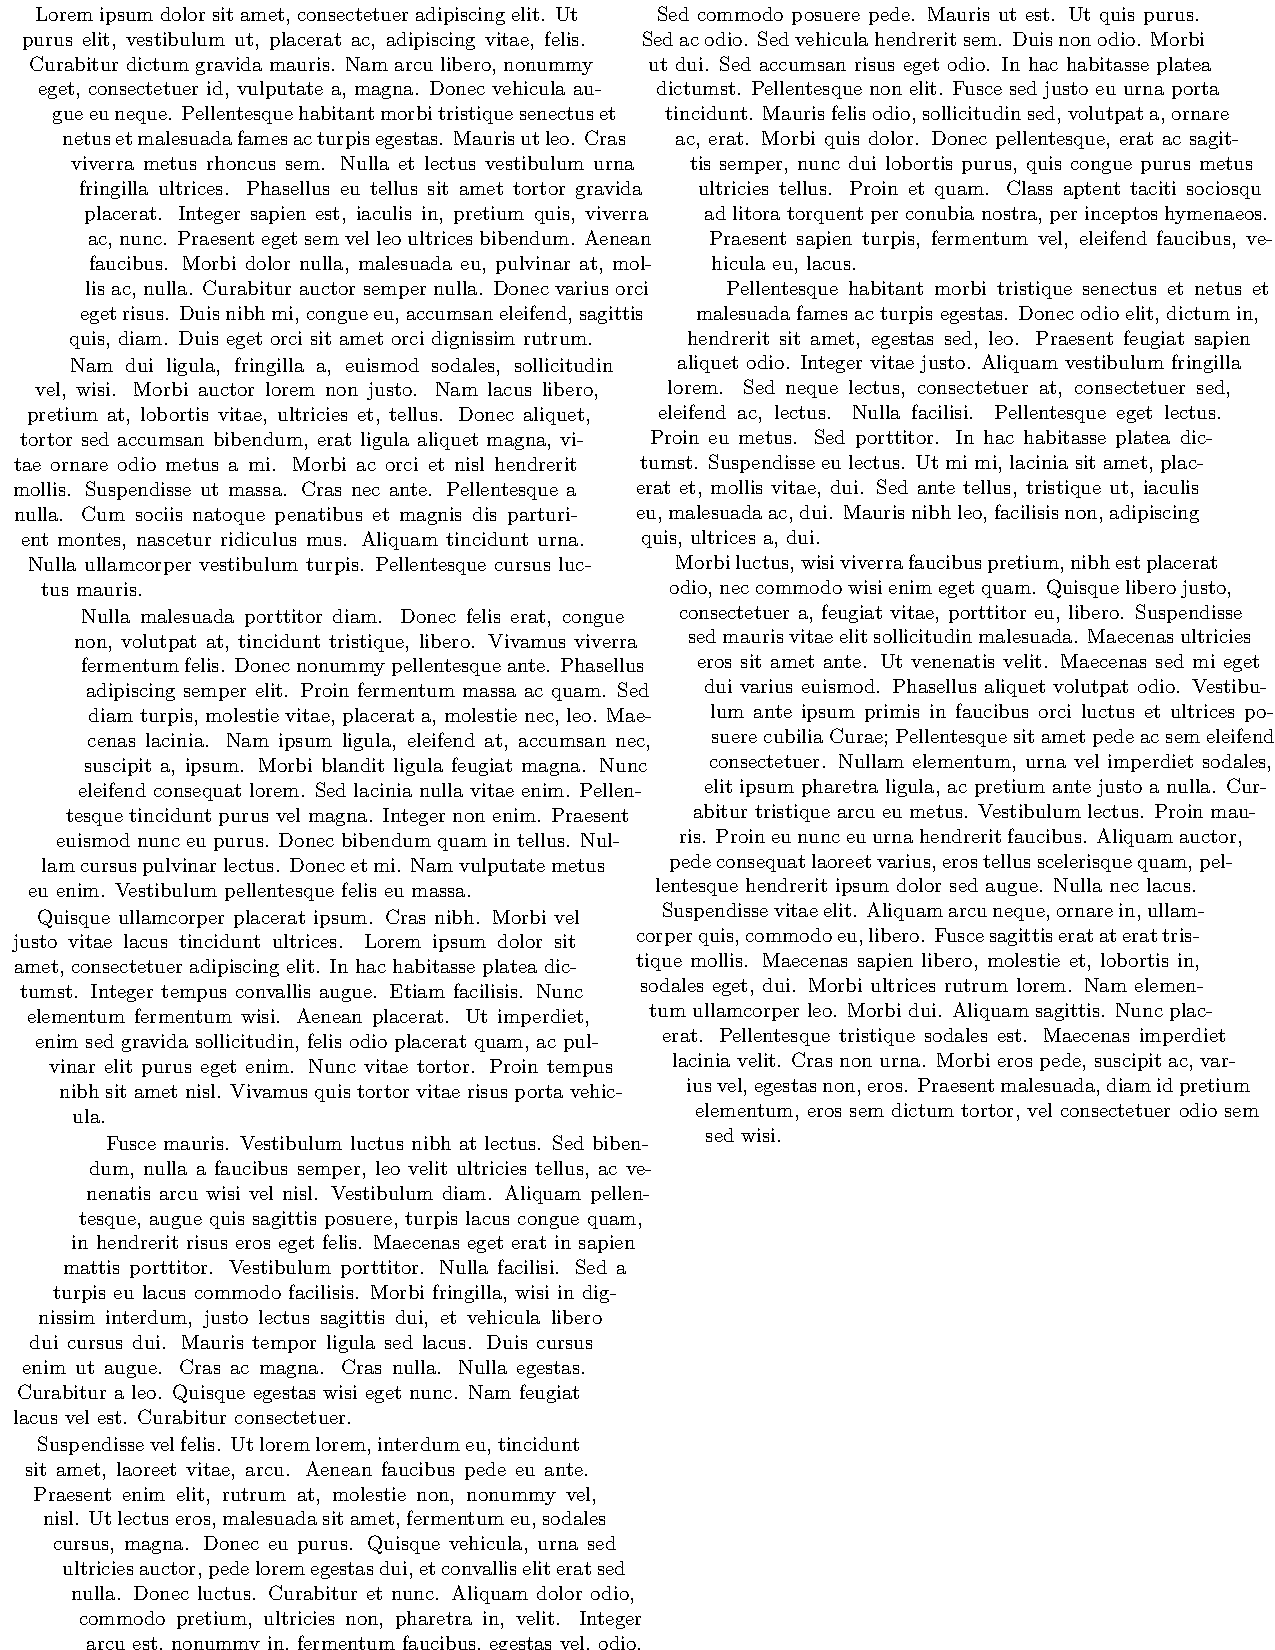
\includegraphics[width=\linewidth, page=1]{lua_example.pdf}
\end{minipage}
\caption{Example of Lua coding\supercite{プログラミングwtTeX}}
\label{fig:lua_ex}
\end{figure}

\subsection{\LaTeX で使える長さについて}
\subsubsection{単位}
\noindent 
長さの単位としてはオーソドックスでなものが多い.
ここで示したもの以外にも様々あるが,使いたい場面がない.

\begin{table}[htbp]
  \caption{List of length units available in \LaTeX.}
  \label{tbl:length_units}
  \centering\begin{tabular}{ccl}\bhline{1pt}
    unit & name & description \\\hline
    pt & point & $1$ pt $\simeq$ $0.35$ mm\\
    pc & pica & $1$ pc $=$ $12$ pt\\
    mm & millimeter & $1$ mm $\simeq$ $2.85$ pt \\
    in & inch & $1$ in $= 25.4$ mm $= 72.27$ pt \\
    em & \textipa{/\textepsilon m/}  &  the width of an ``M'' in the current font \\
    ex & \textipa{/\textepsilon ks/} &  the height of an ``x'' in the current font \\
    zw & zenkaku width &  the width of a zenkaku-kanji in the current font \\
    zh & zenkaku height &  the height of a zenkaku-kanji in the current font \\ \bhline{1pt}
  \end{tabular}
\end{table}

\subsubsection{環境に依存する長さ}
\noindent 一方,環境依存で定義された長さもいくつかある\supercite{layout_doc}.
特に図の挿入時には紙面の横幅に対する割合などを指定すれば,見た目の調整が楽である.
\begin{table}[htbp]
  \begin{minipage}{0.6\linewidth}
    \caption{List of common length macros.}
    \label{tbl:length_macros}
    \centering\begin{tabular}{ll}\bhline{1pt}
      macros & description \\\hline
      \verb|\paperwidth| & width of the page \\
      \verb|\paperheight| & height of the page \\
      \verb|\textwidth| & width of the text on the page \\
      \verb|\textheight| & height of the text on the page \\
      \verb|\linewidth| & width of the line in the current environment \\
      \verb|\columnwidth| & width of the column \\
      \verb|\columnsep| & distance between columns \\
      \verb|\parindent| & indentation of paragraphs \\
      \verb|\parskip| & extra space between paragraphs \\
      \verb|\baselineskip| & vertical distance between lines in a paragraph\\\bhline{1pt}
    \end{tabular}
  \end{minipage}
  \hfill
  \begin{minipage}{0.35\linewidth}
    % \begin{table}[htbp]
      \caption{List of space control macros.}
      \label{tbl:space_control}
      \centering\begin{tabular}{ll}\bhline{1pt}
        macros & definition \\\hline
        \verb*|\ | & $0.33$ em \\
        \verb|~| & $0.33$ em (non-breakable) \\
        \verb|\,| & $3/18$ em\\
        \verb|\:| & $4/18$ em\\
        \verb|\;| & $5/18$ em\\
        \verb|\quad| & $1$ em\\
        \verb|\qquad| & $2$ em\\
        \verb|\!| & $-3/18$ em\\\hline
        \verb|\hspace{}| & flexible horizontal space \\
        \verb|\vspace{}| & vertical\\\bhline{1pt}
      \end{tabular}
    % \end{table}
  \end{minipage}
\end{table}
定義から分かる通り,基本的な長さとしては\verb|\paperwidth|$>$\verb|\textwidth|$\geq$\verb|\linewidth|である.
実際,これらの長さ(の半分)の線を引いてみる\\
\rule{.5\paperwidth}{0.5pt} \verb|.5\paperwidth|\\
\rule{.5\textwidth}{0.5pt} \verb|.5\textwidth| \\
\rule{.5\linewidth}{0.5pt} \verb|.5\linewidth| (in one column)
\setlength{\columnsep}{2em}
\vspace{-10pt}
\begin{multicols}{2}
  \noindent\rule{.5\linewidth}{0.5pt}
  \verb|.5\linewidth| (in 2 cols)\\
  \rule{.5\columnwidth}{0.5pt} \verb|.5\columnwidth|\\
\end{multicols}

\subsubsection{空白}
\noindent 空白の制御を行うときにいつも忘れるのでメモしておく\supercite{spacing_in_LaTeX}.
「カンマ$<$コロン$<$セミコロン」の順に縦に伸びていくので,これで覚えればいいか.


空白関連でもう一つ.
\TeX 処理の際には基本的にピリオドがあると終止符だと認識し,その後ろには大きめの空白が入る.
しかし例外があり,大文字の後ろのピリオドは終止符認識しない(略語などに対応するため).
したがって,大文字の単語が文末にくると,終止符にも関わらず例外として処理されてしまい,次の文との間の空白が本来より小さくなってしまう.
そこでピリオドの直前に大文字以外のなにかを挟めばよいため,例えば\verb|\@. |などが用いられる.


\ifSubfilesClassLoaded{%
  \printbibliography
}% 

\end{document}
